\documentclass{beamer}
\usepackage{amsfonts,amsmath,oldgerm}
\usepackage{ragged2e}
\usepackage[portuguese]{babel}
\DeclareUnicodeCharacter{200B}{I~AM~HERE!!!!}
\usetheme{sintef}

\newcommand{\testcolor}[1]{\colorbox{#1}{\textcolor{#1}{test}}~\texttt{#1}}

\usefonttheme[onlymath]{serif}

\titlebackground*{assets/background}

\newcommand{\hrefcol}[2]{\textcolor{cyan}{\href{#1}{#2}}}

\title{APIs e Swagger}
\subtitle{2023.1 - PDWA5}
\course{Tecnologia em Análise e Desenvolvimento de Sistemas}
\author{\href{mailto:luizfpq@gmail.com}{Luiz \textbf{Quirino}}}
\IDnumber{luizfpq@gmail.com}



\begin{document}
\maketitle

%\begin{frame}
%
%      Este material é produzido utilizando \LaTeX\, baseado na SINTEF Presentation, disponibilizado sob licenciamento \hrefcol{https://creativecommons.org/licenses/by-nc/4.0/legalcode}{Creative Commons CC BY 4.0}
%
%\vspace{\baselineskip}

%In the following you find a brief introduction on how to use \LaTeX\ and the beamer package to prepare slides, based on the one written by \hrefcol{mailto:federico.zenith@sintef.no}{Federico Zenith} for \hrefcol{https://www.overleaf.com/latex/templates/sintef-presentation/jhbhdffczpnx}{SINTEF Presentation}

% This template is released under \hrefcol{https://creativecommons.org/licenses/by-nc/4.0/legalcode}{Creative Commons CC BY 4.0} license

%\end{frame}

\section{Motivação}

\begin{frame}
\frametitle{Relembrando APIs e Swagger}

\begin{itemize}
\item APIs são uma forma de diferentes aplicativos de software se comunicarem entre si.
\item Outras partes podem usar sua API para enviar e recuperar dados sem tocar no código subjacente.
\item O Swagger é um framework de desenvolvimento de API que ajuda a projetar, documentar e testar APIs.
\end{itemize}

\end{frame}
\begin{frame}
\frametitle{Por que o Swagger é importante?}

\begin{itemize}
\item O Swagger simplifica o desenvolvimento de API ao oferecer um ambiente amigável ao usuário.
\item Uma boa documentação é crucial para a adoção de qualquer API e o Swagger ajuda com isso.
\item O Swagger permite que equipes diferentes colaborem na criação de uma API para torná-la mais consistente e eficiente.
\end{itemize}

\end{frame}

\begin{frame}
\frametitle{O processo de design de API}

% \begin{figure}
%   \includegraphics[width=0.8\textwidth]{caminho/do/arquivo}
%   \caption{Processo de design de API.}
% \end{figure}

\begin{itemize}
\item Durante esta fase, você precisa estabelecer a finalidade da sua API, quem irá utilizá-la e definir os endpoints.
\item É crucial pensar em funcionalidade e flexibilidade nesta fase.
\item O processo de design deve ser colaborativo para que diferentes partes interessadas possam fornecer diferentes entradas.
\end{itemize}

\end{frame}

\begin{frame}
\frametitle{Desenvolvimento de API}

% \begin{figure}
%   \includegraphics[width=0.8\textwidth]{caminho/do/arquivo}
%   \caption{Desenvolvimento de API.}
% \end{figure}

\begin{itemize}
\item Esta é a fase de implementação onde você escreve o código e cria endpoints.
\item Testes ajudam a garantir uma boa experiência do usuário.
\item Documente bem seu código para que possa ser usado por outros.
\end{itemize}

\end{frame}

\begin{frame}
\frametitle{Documentação de API}

% \begin{figure}
%   \includegraphics[width=0.8\textwidth]{caminho/do/arquivo}
%   \caption{Documentação de API.}
% \end{figure}

\begin{itemize}
\item Uma boa documentação é essencial, pois serve como referência para outros desenvolvedores.
\item O Swagger fornece ferramentas para ajudar a gerar a documentação automaticamente.
\item Uma documentação bem estruturada facilita para os desenvolvedores utilizarem rapidamente a API.
\end{itemize}

\end{frame}

\begin{frame}
\frametitle{Teste de API}

% \begin{figure}
%   \includegraphics[width=0.8\textwidth]{caminho/do/arquivo}
%   \caption{Teste de API.}
% \end{figure}

\begin{itemize}
\item Testes de API são uma parte crucial do ciclo de desenvolvimento.
\item Testes automatizados minimizam o impacto negativo no ciclo de desenvolvimento no caso de uma funcionalidade quebrar involuntariamente.
\item Swagger torna fácil testar suas APIs usando diferentes consultas e respostas.
\end{itemize}

\end{frame}

\begin{frame}
\frametitle{Simulação e Virtualização de APIs}

% \begin{figure}
%   \includegraphics[width=0.8\textwidth]{caminho/do/arquivo}
%   \caption{Simulação e Virtualização de APIs.}
% \end{figure}

\begin{itemize}
\item A simulação de API ajuda a acelerar os testes e o desenvolvimento.
\item A virtualização permite que os desenvolvedores testem sua API em um cenário real.
\item As ferramentas do Swagger usam um conjunto de critérios ou regras para corresponder solicitações e criar dados simulados.
\end{itemize}

\end{frame}

\begin{frame}
\frametitle{Governança de API}

% \begin{figure}
%   \includegraphics[width=0.8\textwidth]{caminho/do/arquivo}
%   \caption{Governança de API.}
% \end{figure}

\begin{itemize}
\item Governança é o processo de manutenção da qualidade e uso da API.
\item As políticas de governança garantem a conformidade com todos os requisitos técnicos e regulamentações de dados.
\item SwaggerHub fornece um ambiente para implementação, teste, implantação e governança de API.
\end{itemize}

\end{frame}



\begin{frame}
\frametitle{Monitoramento de API}

% \begin{figure}
%   \includegraphics[width=0.8\textwidth]{caminho/do/arquivo}
%   \caption{Monitoramento de API.}
% \end{figure}

\begin{itemize}
\item APIs de monitoramento ajudam a detectar problemas potenciais e permitem melhoria contínua.
\item O monitoramento de desempenho coleta dados ao longo do tempo, com alarmes para disparar se ocorrer uma violação de API.
\item O Swagger fornece uma ferramenta para monitorar a qualidade e o uso do desempenho da API.
\end{itemize}

\end{frame}

\section{Ferramental}

\begin{frame}
\frametitle{Ferramentas OpenAPI e Swagger}

% \begin{figure}
%   \includegraphics[width=0.4\textwidth]{openapi_logo}
%   \caption{Logotipo do OpenAPI.}
% \end{figure}

% \begin{figure}
%   \includegraphics[width=0.2\textwidth]{codegen_logo}
%   \includegraphics[width=0.2\textwidth]{editor_logo}
%   \includegraphics[width=0.2\textwidth]{swagger_ui_logo}
%   \caption{Ferramentas OpenAPI e Swagger: CodeGen, Editor e Swagger UI.}
% \end{figure}

\begin{itemize}
  \item O OpenAPI fornece uma definição de API que funcionará com qualquer linguagem.
  \item O Codegen gera stubs de servidor e SDKs de cliente a partir de especificações OpenAPI.
  \item O Swagger Editor é um editor de código aberto para projetar APIs com as especificações OpenAPI e AsyncAPI.
  \item O Swagger UI ajuda a visualizar uma especificação OpenAPI em uma interface de usuário interativa.
\end{itemize}

\end{frame}

\begin{frame}
  \frametitle{Swagger Open-Source}

    \begin{figure}
      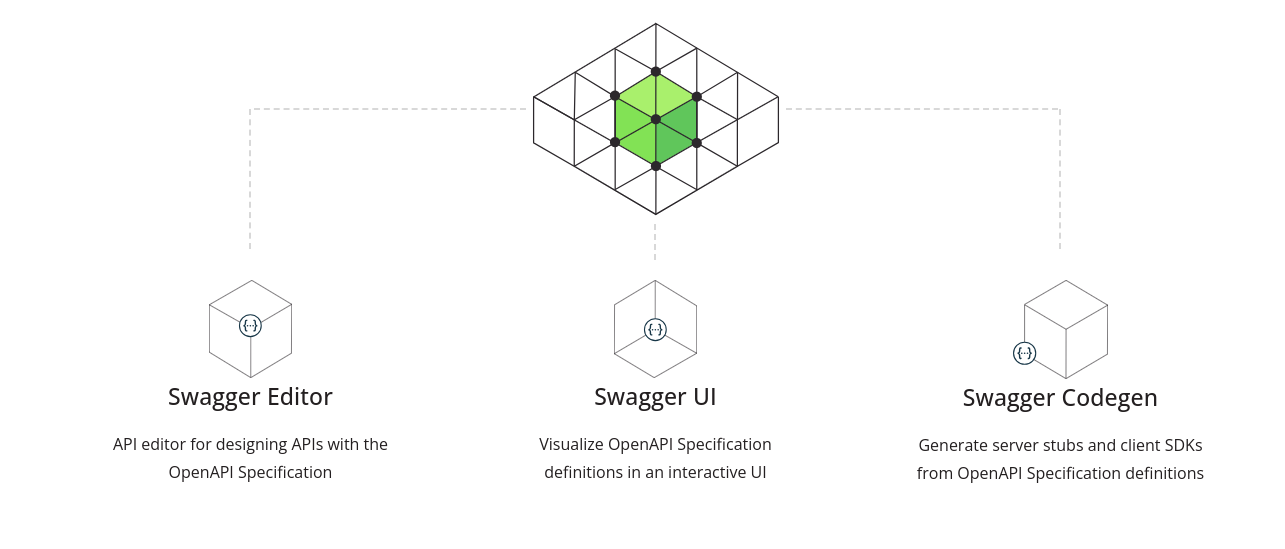
\includegraphics[width=0.8\textwidth]{assets/aula-tads-pdwa5-15-06-2023/SwaggerHub-screenshot.png}
      \caption{Captura de tela do SwaggerHub.}
    \end{figure}

  \end{frame}
    
  

    \begin{frame}
      \frametitle{Swagger Open-Source}    

  \begin{itemize}
    \item O SwaggerHub oferece uma plataforma profissional para o desenvolvimento de sua API.
    \item Todos os membros da equipe podem colaborar facilmente e compartilhar suas APIs.
    \item O SwaggerHub fornece uma variedade de ferramentas como editor de API, verificações de estilo e domínios reutilizáveis para uma API de alta qualidade.
  \end{itemize}
\end{frame}


\begin{frame}
\frametitle{Avalie instantaneamente a funcionalidade de qualquer API}

% \begin{figure}
%   \includegraphics[width=0.8\textwidth]{caminho/do/arquivo}
%   \caption{Captura de tela de um teste de API automático no SwaggerHub.}
% \end{figure}

\begin{itemize}
\item SwaggerHub ajuda a testar a API com diferentes \textit{endpoints}, tornando os testes mais rápidos.
\item Também fornece um design de contrato orientado ao consumidor que permite que membros da equipe gerem testes automaticamente e monitorem serviços.
\item SwaggerHub fornece um ambiente para avaliar a funcionalidade de qualquer API.
\end{itemize}

\end{frame}

\begin{frame}
  \frametitle{Swagger Editor} 
  
  % \begin{figure}
  %   \includegraphics[width=0.8\textwidth]{caminho/do/arquivo}
  %   \caption{Imagem de uma janela de edição no Swagger Editor.}
  % \end{figure}
  
  \begin{itemize}
  \item O Swagger Editor é um editor de código aberto para projetar APIs com OpenAPI ou AsyncAPI.
  \item Ele verifica erros e ajuda a fornecer uma melhor experiência ao usuário.
  \item O Swagger Editor também gera automaticamente a documentação da API.
  \end{itemize}
  
  \end{frame}



  \begin{frame}
    \frametitle{Swagger UI}
    
    % \begin{figure}
    %   \includegraphics[width=0.8\textwidth]{caminho/do/arquivo}
    %   \caption{Captura de tela do Swagger UI em ação.}
    % \end{figure}
    
    \begin{itemize}
    \item O Swagger UI é uma ferramenta de código aberto que ajuda a visualizar uma especificação OpenAPI em uma interface interativa.
    \item Ele fornece documentação detalhada dos pontos finais da API.
    \item O Swagger UI é personalizável para atender às necessidades específicas da sua equipe.
    \end{itemize}
    
    \end{frame}


\begin{frame}
\frametitle{Swagger Codegen}

% \begin{figure}
%   \includegraphics[width=0.8\textwidth]{caminho/do/arquivo}
%   \caption{Captura de tela do processo de geração de código no SwaggerEditor.}
% \end{figure}

\begin{itemize}
\item O Swagger Codegen gera automaticamente código em diferentes linguagens com base em definições de API.
\item Ajuda a reduzir o tempo de desenvolvimento do código.
\item O Swagger Codegen fornece bibliotecas adicionais e SDKs.
\end{itemize}
\end{frame}


\begin{frame}

\frametitle{Recursos}

% \begin{figure}
%   \includegraphics[width=0.8\textwidth]{caminho/do/arquivo}
%   \caption{Captura de tela do site e documentação do Swagger.}
% \end{figure}

\begin{itemize}
\item A documentação da especificação do OpenAPI é um bom ponto de partida para aprender mais sobre documentação de API.
\item O site do Swagger fornece ferramentas e conselhos sobre como melhorar o processo de desenvolvimento de API.
\item Recursos sobre APIs, Swagger e OpenAPI estão amplamente disponíveis.
\end{itemize}

\end{frame}

\begin{frame}

\frametitle{Documentação da Especificação do OpenAPI}

% \begin{figure}
%   \includegraphics[width=0.8\textwidth]{caminho/do/arquivo}
%   \caption{Captura de tela da documentação da especificação do OpenAPI.}
% \end{figure}

\begin{itemize}
\item A especificação OpenAPI ajuda a definir APIs.
\item A especificação é escrita em YAML, um formato legível por humanos.
\item A especificação fornece uma descrição dos endpoints da API e das respostas esperadas.
\end{itemize}

\end{frame}

\begin{frame}
  \frametitle{Suporte do Swagger}
  
  % \begin{figure}
  %   \includegraphics[width=0.8\textwidth]{caminho/do/arquivo}
  %   \caption{Captura de tela do site de suporte.}
  % \end{figure}
  
  \begin{itemize}
    \item SmartBear fornece suporte para usuários do Swagger.
    \item O suporte inclui documentação, guias e tutoriais.
  \end{itemize}
  
  \end{frame}
  

\begin{frame}
  \frametitle{Blog do Swagger}
  
  % \begin{figure}
  %   \includegraphics[width=0.8\textwidth]{caminho/do/arquivo}
  %   \caption{Captura de tela da página do blog no site Swagger.}
  % \end{figure}
  
  \begin{itemize}
    \item O blog Swagger fornece insights sobre desenvolvimento e gerenciamento de APIs.
    \item O blog apresenta artigos escritos por especialistas em desenvolvimento e gerenciamento de APIs.
    \item O blog fornece as últimas notícias em desenvolvimento e gerenciamento de APIs.
  \end{itemize}
  
  \end{frame}
  

  \begin{frame}
    \frametitle{Conclusão}
    
    % \begin{figure}
    %   \includegraphics[width=0.6\textwidth]{caminho/do/arquivo}
    %   \caption{Imagem de pessoas celebrando.}
    % \end{figure}
    
    \begin{itemize}
      \item As APIs são cruciais para o desenvolvimento de software, e o Swagger ajuda a simplificar o processo de desenvolvimento.
      \item Uma boa documentação é essencial, e o Swagger ajuda a fornecer um ambiente colaborativo.
      \item O Swagger fornece um conjunto de ferramentas para design, desenvolvimento, teste e documentação de APIs REST.
    \end{itemize}
    
    \end{frame}
    
    \begin{frame}
      \frametitle{Referências}
      
      \begin{itemize}
        \item Swagger: Documentação oficial. Disponível em: \url{https://swagger.io/docs/}
        \item OpenAPI: Recursos de aprendizado. Disponível em: \url{https://learn.openapis.org/}
        \item Swagger UI React: Pacote npm para integração do Swagger UI com React. Disponível em: \url{https://www.npmjs.com/package/swagger-ui-react}
      \end{itemize}
      
      \end{frame}
      
                                
\backmatter
\end{document}
